\part{Ideation}
\frame{\partpage}

\begin{frame}{Intro}
	\begin{itemize}
		\item Seen as one of the most important stages
		\item Used to generate challenges
		\item Allows you to explore the possibility space
		\item Challenge assumptions about an area
	\end{itemize}
\end{frame}

\begin{frame}{Brainstorming}
	\begin{columns}
		\begin{column}{0.48\textwidth}
			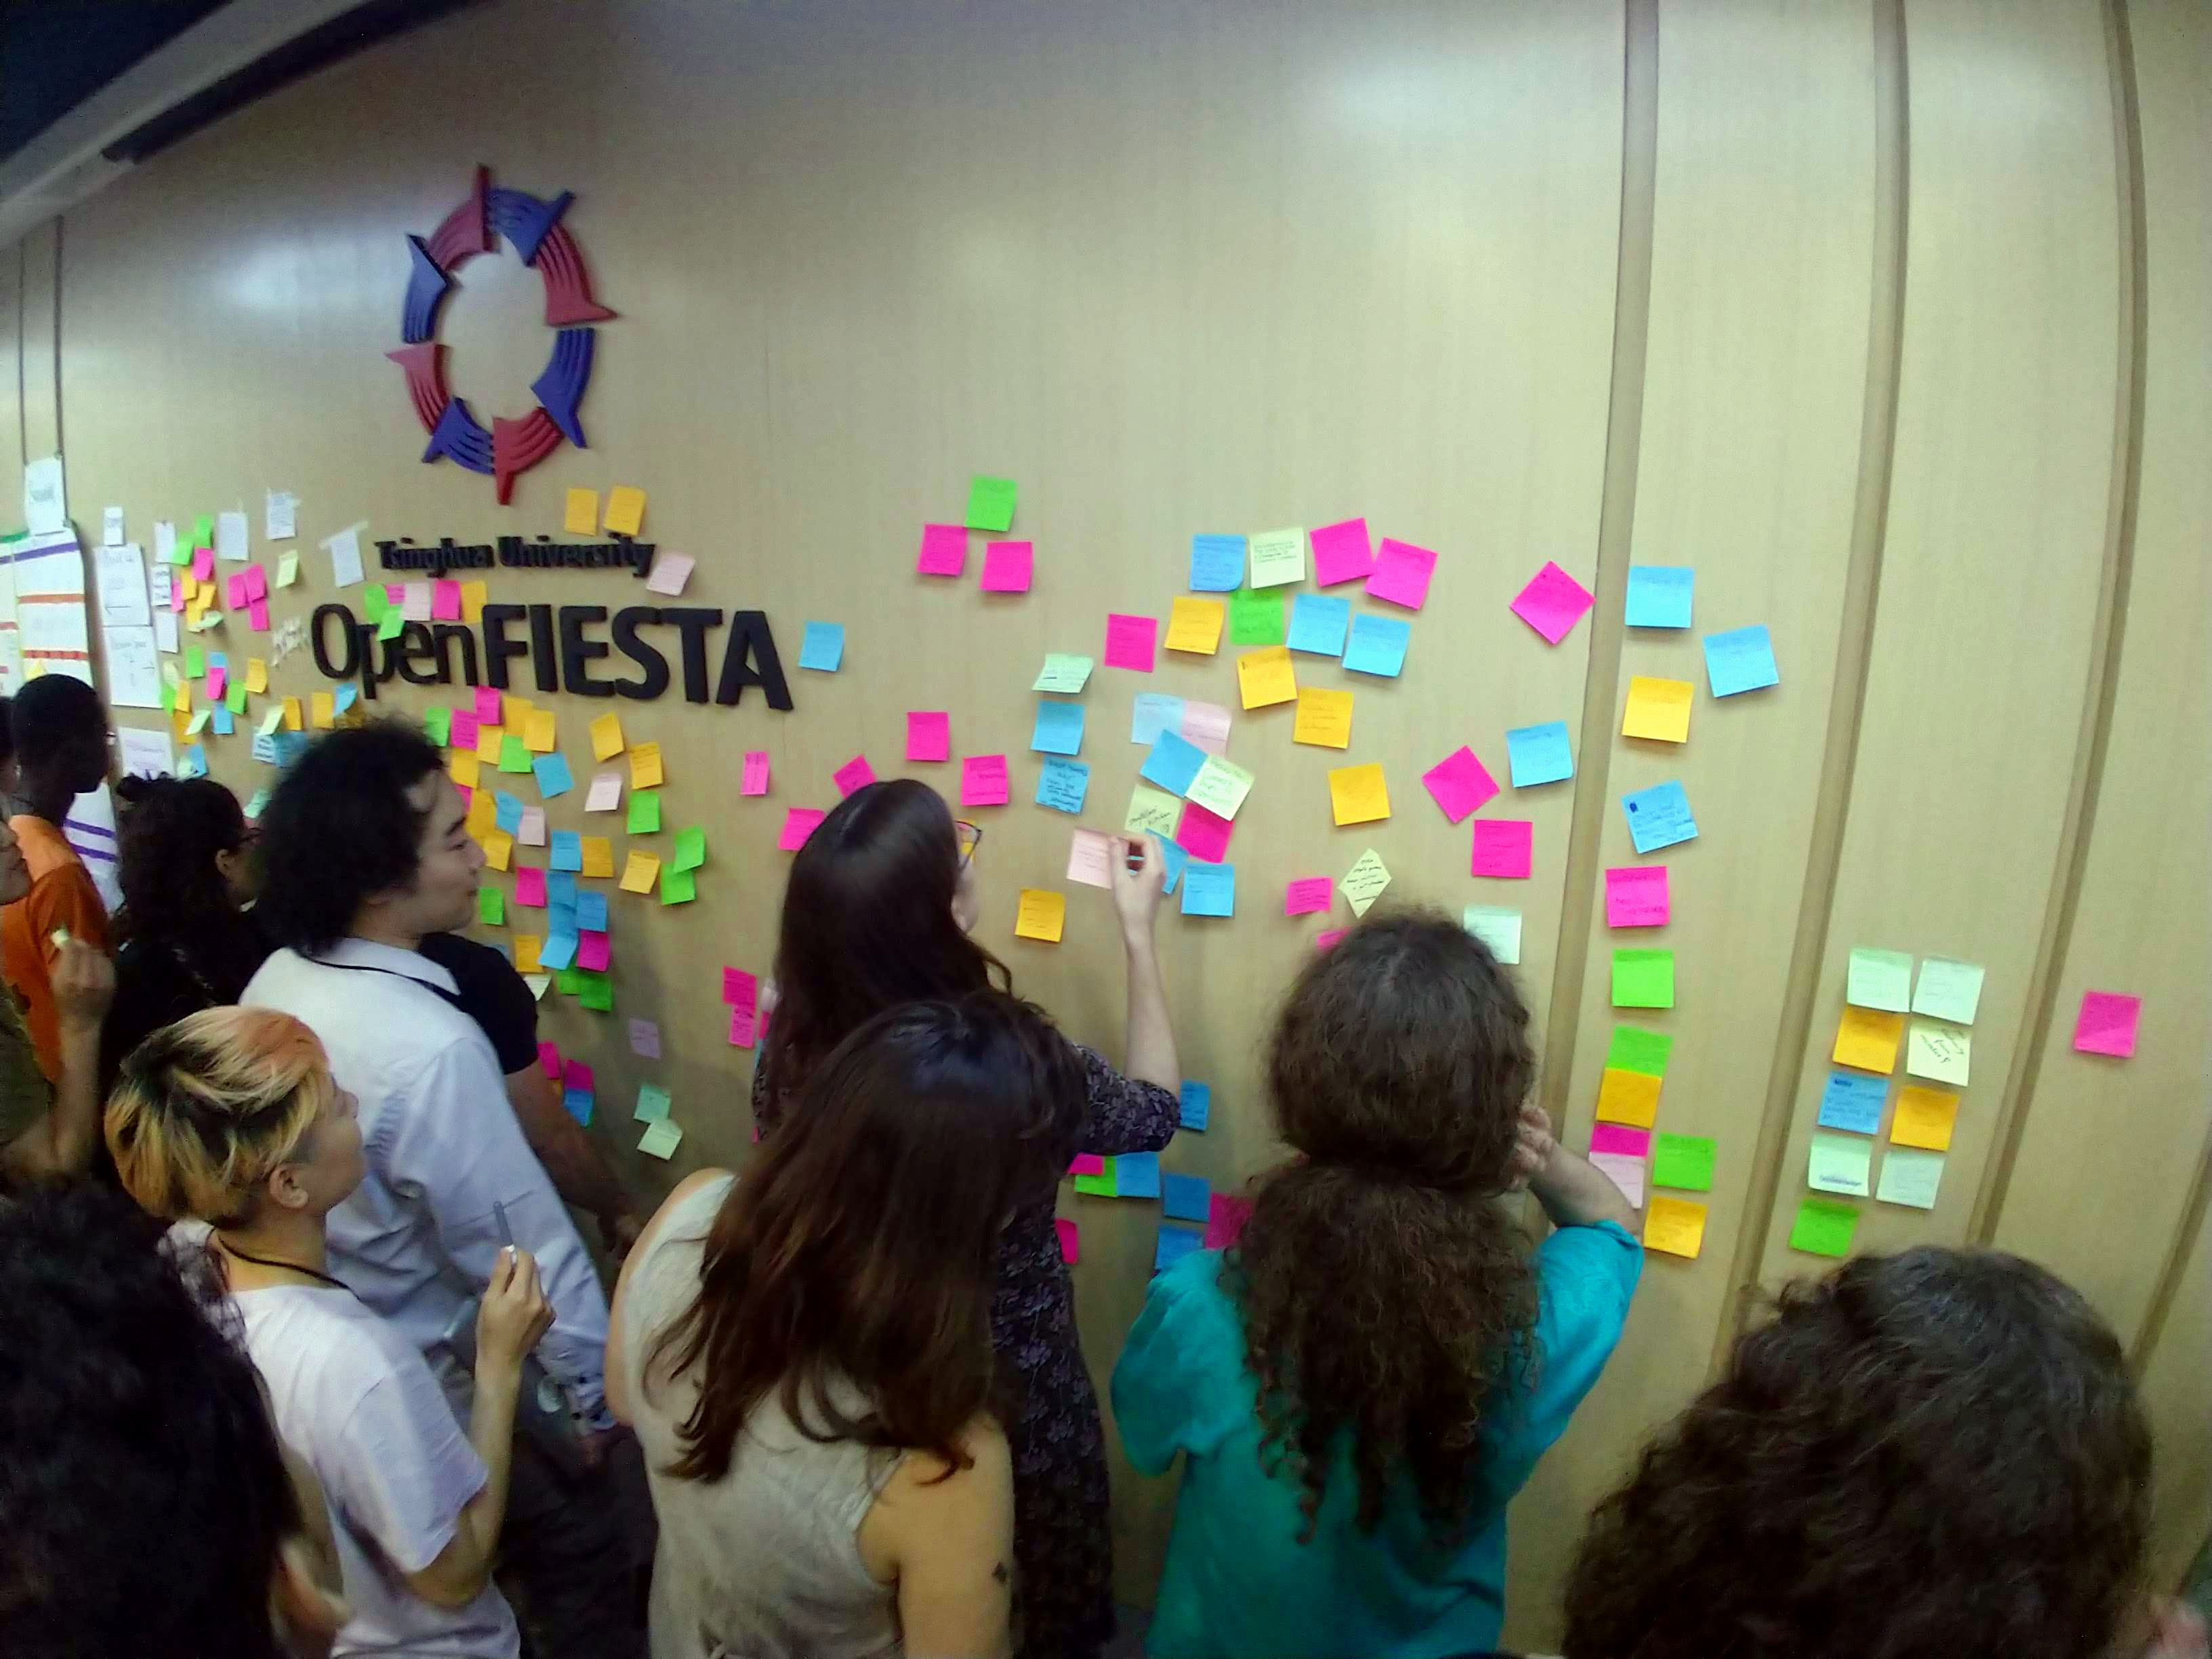
\includegraphics[width=0.9\textwidth, height=0.7\textheight]{brain_storming}
		\end{column}
		\begin{column}{0.48\textwidth}
			\begin{itemize}
				\item First described by Alex Osborn(1953)
			\end{itemize}
			\begin{enumerate}
				\item Idea Quantity
				\item Criticism of the ideas withheld
				\item Wilder the idea, the better
				\item Combine and Improvement
			\end{enumerate}
		\end{column}
	\end{columns}
\end{frame}

\begin{frame}{List Creation}
	\begin{columns}
		\begin{column}{0.48\textwidth}
			\begin{itemize}
				\item Write everything you can about a topic
				\item Free association allows you to explore the area
				\item While organisation of the list allows you to explore relationships 
			\end{itemize}
		\end{column}
		\begin{column}{0.48\textwidth}
			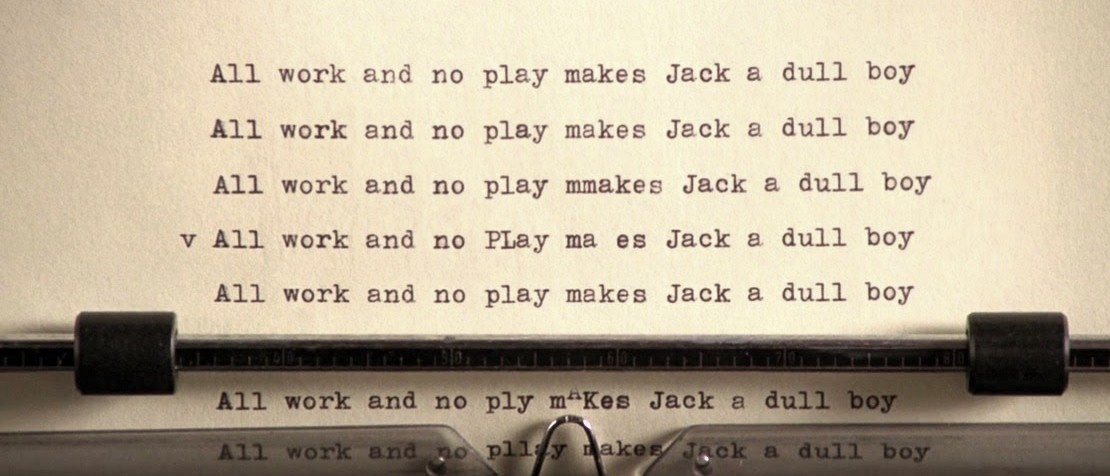
\includegraphics[width=0.9\textwidth, height=0.7\textheight]{list_creation}
		\end{column}
	\end{columns}
\end{frame}

\begin{frame}{Idea/Creativity Cards}
	\begin{columns}
		\begin{column}{0.48\textwidth}
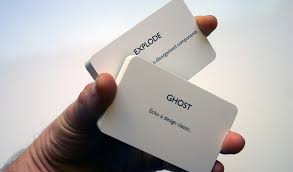
\includegraphics[width=0.9\textwidth, height=0.7\textheight]{creativity_cards}	
		\end{column}
		\begin{column}{0.48\textwidth}
			\begin{itemize}
				\item Start with a blank deck of index cards
				\item Write words on each one
				\item Shuffle the deck, draw two and pair them
				\item Rinse repeat
				\item Or use Creativity Cards
			\end{itemize}
		\end{column}
	\end{columns}
\end{frame}

\begin{frame}{Mind Maps}
	\begin{columns}
		\begin{column}{0.48\textwidth}
			\begin{itemize}
				\item Part of a family of techniques known as \textbf{Concept Mapping}
				\item Demonstrates how people can visualise relationships between topics
				\item Useful for generating a game grammar
			\end{itemize}
		\end{column}
		\begin{column}{0.48\textwidth}
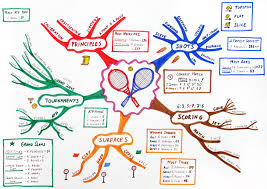
\includegraphics[width=0.9\textwidth, height=0.7\textheight]{mind_map}
		\end{column}
	\end{columns}
\end{frame}

\begin{frame}{Stream of Conscious}
	\begin{columns}
		\begin{column}{0.48\textwidth}
			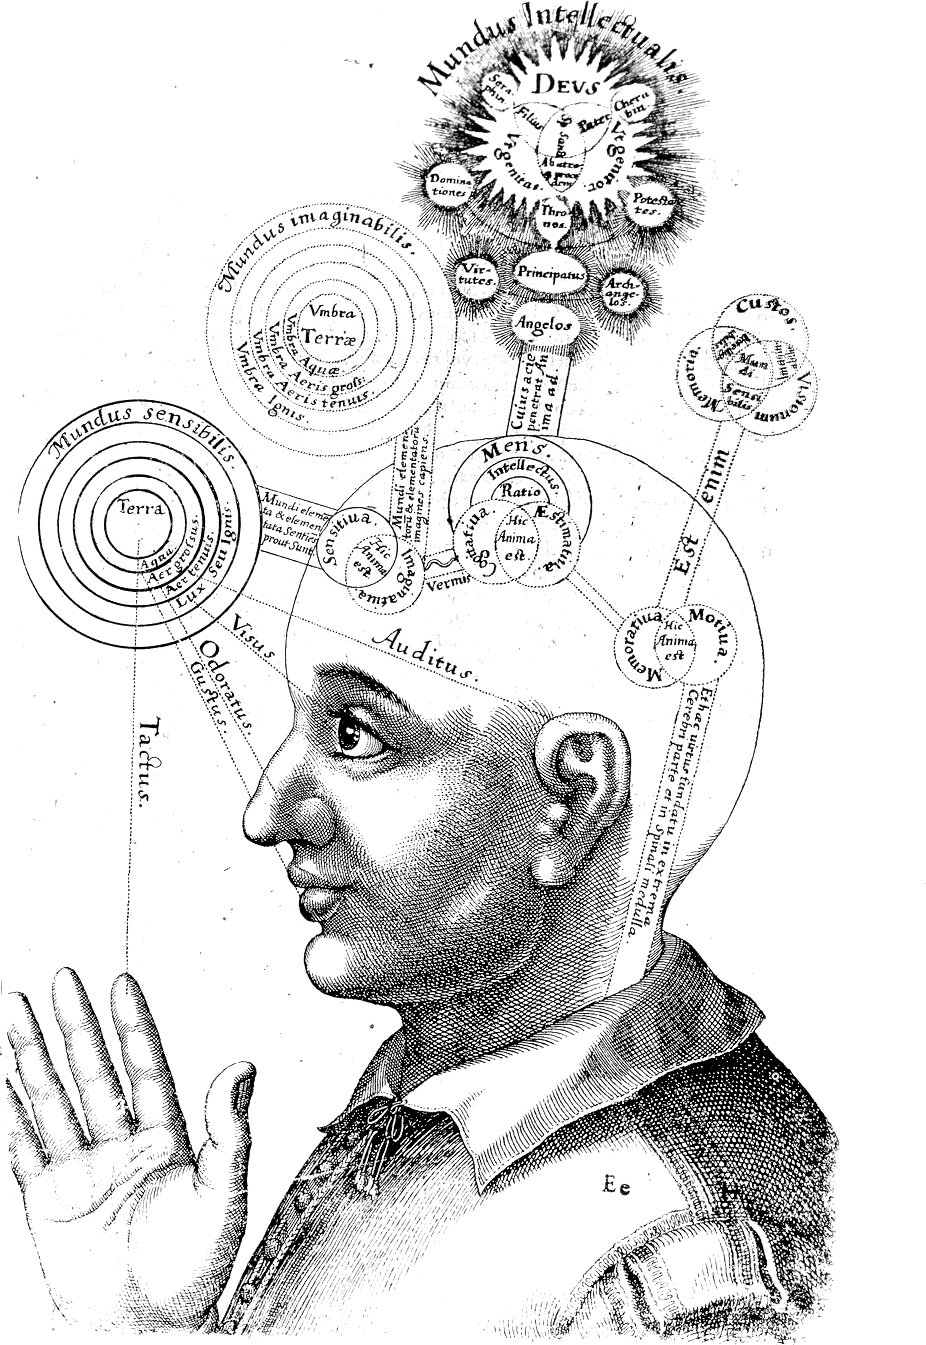
\includegraphics[width=0.9\textwidth, height=0.7\textheight]{stream_of_conscious}
		\end{column}
		\begin{column}{0.48\textwidth}
			\begin{itemize}
				\item Sit down at a computer (or with pen \& paper)
				\item Write everything that comes in mind for 10 mins
				\item Shout out is a variation, which you speak into a voice recorder for 10 mins
			\end{itemize}
		\end{column}
	\end{columns}
\end{frame}

\begin{frame}{Cut it Up}
	\begin{columns}
		\begin{column}{0.48\textwidth}
			\begin{itemize}
				\item Used by the Dadaist art movement e.g. How to Make a Dadaist Poem by Tristan Tzara
				\item Take a magazine or newspaper, cut out word and images
				\item Start playing with pieces and arranging to form ideas
				\item Can lead to surreal juxtapositions 
			\end{itemize}
		\end{column}
		\begin{column}{0.48\textwidth}
			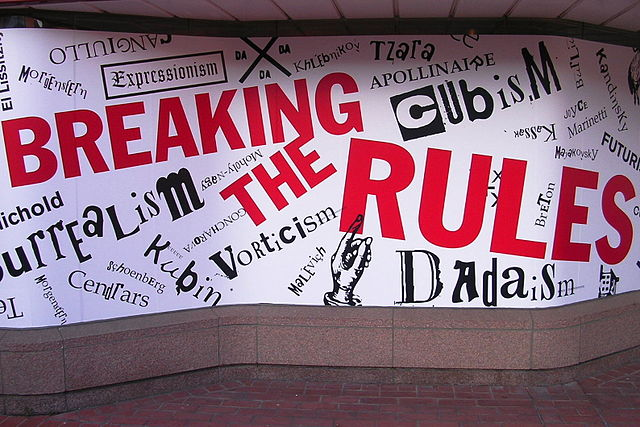
\includegraphics[width=0.9\textwidth, height=0.7\textheight]{cut_up}
		\end{column}
	\end{columns}
\end{frame}

\begin{frame}{Research}
	\begin{columns}
		\begin{column}{0.48\textwidth}
			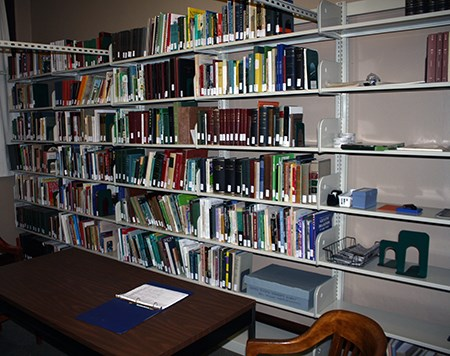
\includegraphics[width=0.9\textwidth, height=0.7\textheight]{research}
		\end{column}
		\begin{column}{0.48\textwidth}
			\begin{itemize}
				\item  Useful for serious games and games that are grounded in a world
				\item Research a topic that interests you. Immerse yourself in a topic
				\item Even if your game isn’t ground in the real world it might have real world analogues
				
			\end{itemize}
		\end{column}
	\end{columns}
\end{frame}